\documentclass[10pt]{article}
\usepackage[polish]{babel}
\usepackage[utf8]{inputenc}
\usepackage[T1]{fontenc}
\usepackage{graphicx}
\usepackage[export]{adjustbox}
\graphicspath{ {./images/} }
\usepackage{amsmath}
\usepackage{amsfonts}
\usepackage{amssymb}
\usepackage[version=4]{mhchem}
\usepackage{stmaryrd}

\title{VIII Konkurs matematyczny St@ś }

\author{}
\date{}


\begin{document}
\maketitle
XIV LO im. Stanisława Staszica 2 czerwca 2008 roku

\section*{klasa VI}
Na rozwiazanie poniższych zadań masz 90 minut.\\
Kolejność rozwiqzywania tych zadań jest dowolna.\\
Wszystkie zadania sa jednakowo punktowane.\\
Maksymalna liczbę punktów może uzyskać jedynie petne rozwiqzanie, z uzasadnieniem i odpowiedziq.\\
Uzywanie korektora i korzystanie z kalkulatora jest niedozwolone.

\section*{Zadanie 1.}
Przerysuj krzyżówkę i tak ją uzupełnij, aby otrzymane liczby trzycyfrowe dzieliły się przez liczby z szarych pól.\\
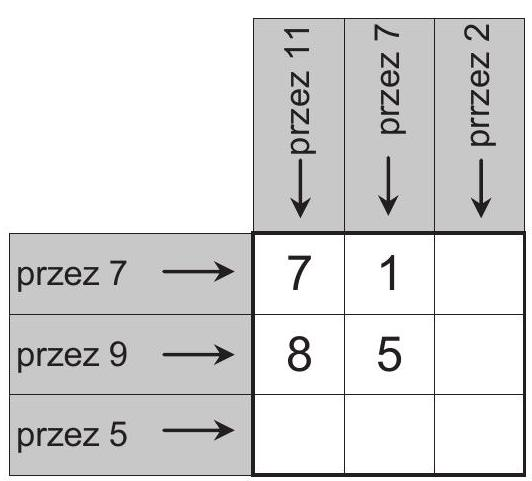
\includegraphics[max width=\textwidth, center]{2024_11_21_f8e9b6ddbb018da21a54g-1(1)}

\section*{Zadanie 2.}
Dany jest trapez \(A B C D\) o podstawach \(A B\) i \(C D\). W tym trapezie \(|A D|=|D C| \mathrm{i}|A C|=|C B|\). Kąt \(A C B\) ma miarę \(88^{\circ}\). Oblicz miarę kąta \(A D C\).

\section*{Zadanie 3.}
Podaj przykład takiej liczby dziewięciocyfrowej, której suma cyfr jest równa 4, i która jest kwadratem liczby naturalnej. Podaj jeszcze dwa inne przykłady takich liczb.\\
Uzasadnij, że Twoje przykłady są prawidłowe.

\section*{Zadanie 4.}
Dany jest taki prostopadłościan, w którym suma pól pewnych dwóch ścian jest większa od sumy pól pozostałych czterech ścian. Uzasadnij, że te dwie ściany to ściany równoległe.

\section*{Zadanie 5.}
Z ośmiu kart ułożono dwa dodawania poziomo i dwa dodawania pionowo. Na każdej karcie jest liczba całkowita, ale niektóre karty nie zostały odkryte. Znajdź liczbę na szarej karcie. Uzasadnij swoją odpowiedź.\\
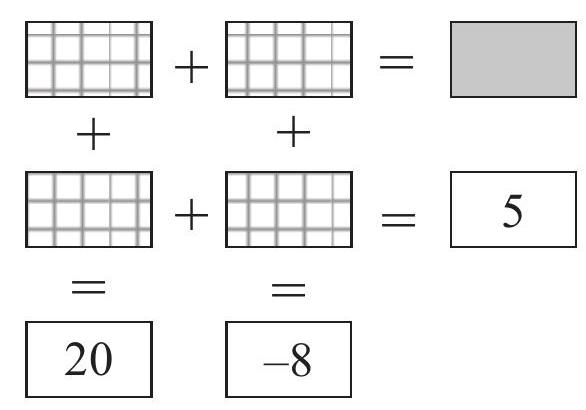
\includegraphics[max width=\textwidth, center]{2024_11_21_f8e9b6ddbb018da21a54g-1}


\end{document}